%% 
%% Copyright 2007-2024 Elsevier Ltd
%% 
%% This file is part of the 'Elsarticle Bundle'.
%% ---------------------------------------------
%% 
%% It may be distributed under the conditions of the LaTeX Project Public
%% License, either version 1.3 of this license or (at your option) any
%% later version.  The latest version of this license is in
%%    http://www.latex-project.org/lppl.txt
%% and version 1.3 or later is part of all distributions of LaTeX
%% version 1999/12/01 or later.
%% 
%% The list of all files belonging to the 'Elsarticle Bundle' is
%% given in the file `manifest.txt'.
%% 
%% Template article for Elsevier's document class `elsarticle'
%% with harvard style bibliographic references

\documentclass[preprint,12pt,authoryear]{elsarticle}
\usepackage{graphicx}      % include this line if your document contains figures
\usepackage{hyperref}
\usepackage{natbib}        % required for bibliography
%\usepackage{amsfonts}
\usepackage{tabularx}
\usepackage{caption}
%\usepackage{amssymb}
\usepackage{amsmath}
\usepackage{mathtools}
\usepackage{siunitx}
\usepackage{subfigure}
\usepackage{algorithm}
%\usepackage{algpseudocode}
\usepackage{booktabs}
\usepackage{url}
\usepackage{cite}
\usepackage{amsmath,amssymb,amsfonts}
\usepackage{algorithmic}
\usepackage{graphicx}
\usepackage{textcomp}
\usepackage{xcolor}
\usepackage{float}
\def\BibTeX{{\rm B\kern-.05em{\sc i\kern-.025em b}\kern-.08em
    T\kern-.1667em\lower.7ex\hbox{E}\kern-.125emX}}

\DeclareMathOperator{\argmin}{arg\;min}
\DeclareMathOperator{\vol}{vol}
\DeclareMathOperator{\diag}{diag}
\newcommand{\ui}[2]{#1_{\text{#2}}}
\newcommand{\uis}[2]{#1^{\text{#2}}}
\newcommand{\lrp}[1]{\left( #1 \right)}
\newcommand{\uib}[2]{{\bf #1}_{\text #2}}
\newcommand{\Ts}{\ui{T}{s}}

%% NN controller commands
\newcommand{\cnn}{\ui{\mathcal{C}}{NN}}
\newcommand{\fddpg}{\ui{f}{E}}
\newcommand{\uddpg}{\ui{u}{E}}
\newcommand{\actor}{\ui{f}{ACT}}
\newcommand{\critic}{\ui{f}{CRIT}}
\newcommand{\thx}{\ui{\theta}{x}}
\newcommand{\thf}{\ui{\theta}{f}}
\newcommand{\ucorr}{\widetilde{u}}
\newcommand{\unn}{\ui{u}{nn}}
\newcommand{\uact}{\ui{u}{ACT}}
\newcommand{\corr}{\ui{\mathcal{C}}{C}}
\newcommand{\todo}[1]{{{\color{red} TODO: #1	}} }
\renewcommand{\mark}[1]{{{\color{green} #1	}} }
%\newcommand{\e}[1]{\cdot 10^{#1}}
%%-------------------------------------------------------
%% MACRO for tikz picture. DO NOT CHANGE ANYTHING !!!!!
\usepackage{tikz}
\usepackage{pgfkeys}
\usepackage{calc}
\usepackage{pgfplots}
\usetikzlibrary{arrows}
\usetikzlibrary{calc}
\usepgflibrary{arrows}
\usetikzlibrary{positioning}
\usetikzlibrary{intersections}
\pgfplotsset{compat=newest}
\usetikzlibrary{shapes.geometric}
\usetikzlibrary{decorations.pathreplacing}
\usetikzlibrary{patterns,decorations.pathmorphing,decorations.markings}
\usetikzlibrary{external}
\usetikzlibrary{plotmarks}
\usetikzlibrary{arrows.meta}
\usepgfplotslibrary{patchplots}
\usepackage{grffile}
\usepgfplotslibrary{fillbetween}
\usepackage{xfrac}
%\tikzexternalize
\newcommand{\R}{\mathbb{R}}
\newcommand{\includetikz}[1]{%
\tikzifexternalizing{%
\def\DOIT{1}%
}{%
\IfFileExists{#1.pdf}{%
\includegraphics[scale=1]{#1.pdf}%
\def\DOIT{0}%
}{%
\def\DOIT{1}%
}%
}%
%
\if1\DOIT
%	\tikzsetnextfilename{mypic_#1}%
\tikzsetnextfilename{#1}
%   \filemodCmp{#1.tikz}{external/#1.log}%
%  {\tikzset{external/force remake=true}\input{#1.tikz}}
\input{#1.tikz}
\fi
}

% defines lengths for figure plotting
\newlength\figureheight
\newlength\figurewidth
%%  End of TikZ Macros
%%-------------------------------------------------------
\begin{document}

\begin{frontmatter}

%% Title, authors and addresses

%% use the tnoteref command within \title for footnotes;
%% use the tnotetext command for theassociated footnote;
%% use the fnref command within \author or \affiliation for footnotes;
%% use the fntext command for theassociated footnote;
%% use the corref command within \author for corresponding author footnotes;
%% use the cortext command for theassociated footnote;
%% use the ead command for the email address,
%% and the form \ead[url] for the home page:
%% \title{Title\tnoteref{label1}}
%% \tnotetext[label1]{}
%% \author{Name\corref{cor1}\fnref{label2}}
%% \ead{email address}
%% \ead[url]{home page}
%% \fntext[label2]{}
%% \cortext[cor1]{}
%% \affiliation{organization={},
%%            addressline={}, 
%%            city={},
%%            postcode={}, 
%%            state={},
%%            country={}}
%% \fntext[label3]{}

\title{The Beggining of Control Revolution: Ofset-free Koopman MPC} %% Article title

%% use optional labels to link authors explicitly to addresses:
%% \author[label1,label2]{}
%% \affiliation[label1]{organization={},
%%             addressline={},
%%             city={},
%%             postcode={},
%%             state={},
%%             country={}}
%%
%% \affiliation[label2]{organization={},
%%             addressline={},
%%             city={},
%%             postcode={},
%%             state={},
%%             country={}}

\author{Patrik Valábek} %% Author name

%% Author affiliation
\affiliation{organization={STU},%Department and Organization
            addressline={Redlinskeho 9}, 
            city={Bratislava},
            country={Slovakia}}

%% Abstract
\begin{abstract}
%% Text of abstract

\end{abstract}

%%Graphical abstract
%\begin{graphicalabstract}
%\includegraphics{grabs}
%\end{graphicalabstract}

%%Research highlights
\begin{highlights}
\item Research highlight 1
\item Research highlight 2
\end{highlights}

%% Keywords
\begin{keyword}
%% keywords here, in the form: keyword \sep keyword

%% PACS codes here, in the form: \PACS code \sep code

%% MSC codes here, in the form: \MSC code \sep code
%% or \MSC[2008] code \sep code (2000 is the default)

\end{keyword}

\end{frontmatter}

%% Add \usepackage{lineno} before \begin{document} and uncomment 
%% following line to enable line numbers
%% \linenumbers

%% main text
%%
\section{Introduction}
\label{sec:intro}

\section{Preliminaries and Notation}
\label{sec:Preliminaries}

\subsection{Parsim-K Identification}
 
\subsection{Offset-Free MPC}

\subsection{Nonlinear MPC}

\subsection{Koopman Operator for Control}

\subsection{Koopman MPC}

\subsection{State Estimation - Observer}

\section{Koopman MPC with Offset-Free - Easyiest}
\label{sec:easy-mpc}
In this section, we will present a standard offset free optimal framework consisting of Target Optimization, State Estimation - Observer and MPC. As observer is standard Kalman filter or extended Kalman filter, we will discuss mainly remaining two optimization problems. Both remaining components had to be designed in a way that they are able to work with the Koopman operator. The main goal of this section is to show that the standard formulation can be easily transformed for the offset-free MPC use.

\begin{figure}[H]
  \centering
  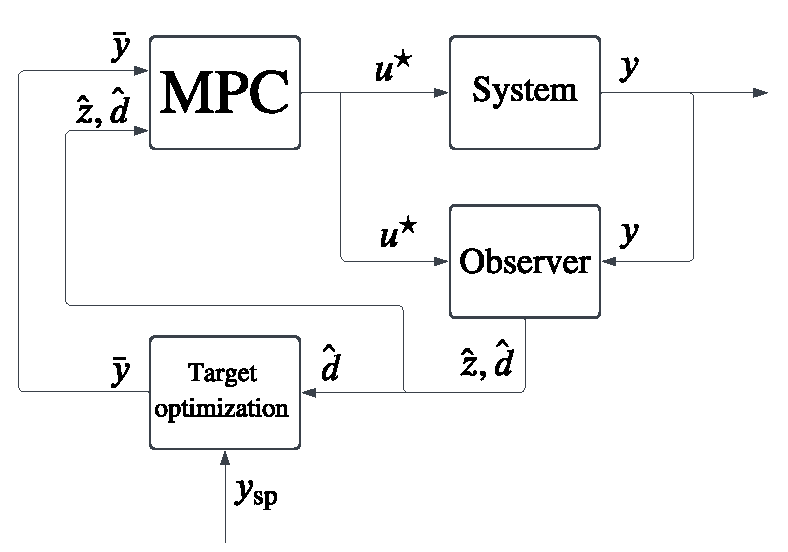
\includegraphics[width=0.95\linewidth]{figures/close_loop.pdf}
  \caption{Closed-loop control structure.}
  \label{fig:close_loop}
\end{figure}

\subsection{Target Optimization}

\begin{subequations}
  \label{eq:target:opt}
  \begin{align}
    \min_{\bar{u}, \bar{z}, \bar{y}} \quad & \; (\bar{y} - y_\text{ref})^\intercal Q_\text{y} (\bar{y} - y_\text{ref}) \label{eq:target:opt:obj} \\
    \text{s.t.} \quad & \; \bar{z} = A\bar{z} + B\bar{u} \label{eq:target:opt:z} \\
    & \; \bar{y} = C\bar{z} + d \label{eq:target:opt:y} \\
    & \; u_{\min} \leq \bar{u} \leq u_{\max} \label{eq:target:opt:u} \\
    & \; y_{\min} \leq \bar{y} \leq y_{\max} \label{eq:target:opt:ycon} \\
    & \; d = \hat{d}(t), \quad y_\text{ref} = y_\text{sp} \label{eq:target:opt:params}
  \end{align}
\end{subequations}



\subsection{MPC}
\begin{subequations}
  \label{eq:of:mpc}
  \begin{align}
    \min_{u_0, \ldots, u_{N-1}} \; & \; \sum_{k=0}^{N-1} (y_k - \bar{y})^\intercal Q_\text{y} (y_k - \bar{y}) + \sum_{k=0}^{N-1} \Delta u_k^\intercal Q_\text{u} \Delta u_k, \label{eq:of:mpc:obj} \\
    \text{s.t.} \;\;\;\; & \; z_{k+1} = A z_k + B u_k, \quad k\in\mathbb{N}_0^{N-1}, \label{eq:of:mpc:z} \\
    & \; y_k = C z_k + d, \quad k\in\mathbb{N}_0^{N-1}, \label{eq:of:mpc:y} \\
    & \; \Delta u_k = u_k - u_{k-1}, \quad k\in\mathbb{N}_0^{N-1}, \label{eq:of:mpc:du} \\
    & \; u_{\min} \leq u_k \leq u_{\max}, \quad k\in\mathbb{N}_0^{N-1}, \label{eq:of:mpc:u} \\
    & \; y_{\min} \leq y_k \leq y_{\max}, \quad k\in\mathbb{N}_0^{N-1}, \label{eq:of:mpc:ycon} \\
    & \; z_0 = \hat{z}(t), \quad d = \hat{d}(t), \quad u_{-1} = u(t-T_\text{s}) \label{eq:of:mpc:init}
  \end{align}
\end{subequations}

\subsection{Closed-Loop Control Structure}

\section{Koopman MPC with Offset-Free - Proposed}

Main drawback that we observe in a current Koopman MPC (offset-free, robust, or any other), is that the optimization is done without leveraging knowledge of the lifted space. Of course we are predicting in the lifted space, but in objective function we are using original space, that is created derived as linear transformation of the lifted space \(y_k = Cz_k\). This transformation is not linear by nature \(y_k = h(z_k)\), but to use linear MPC, we think we had no other choice. Some papers are not using this transformation directly, but after closer look, they are usually using equivalent transformations, for example expanding lifted space with measurements, but dynamic in lifted space is linear, so transformations to achieve back this measurements is linear. We will show that we can use the lifted space directly in the objective function, showing how to handle the lifted space and transformation of an objective function.
We can fully eliminate the neccessity of the back transformation used in objective function in MPC, but we still need them to compute the target for the lifted space. In this case and case of constraints, we use a first order Taylor expansion, to better approximate the transformation. 

\subsection{Target Optimization}

The objective function of target estimation is the same as in the standard offset-free MPC. The main difference is in 

The proposed target optimization problem is formulated as:

\begin{subequations}
  \label{eq:cs:target}
  \begin{align}
    \min_{\bar{u}, \bar{z}, \bar{y}} \quad & \; (\bar{y} - y_\text{ref})^\intercal Q_\text{y} (\bar{y} - y_\text{ref}), \label{eq:cs:target:obj} \\
    \text{s.t.} \quad & \; \bar{z} = A\bar{z} + B\bar{u}, \label{eq:cs:target:z} \\
    & \; \bar{y} = H(\ui{z}{LP})\bar{z} + h(\ui{z}{LP}) - H(\ui{z}{LP})\ui{z}{LP} + d, \label{eq:cs:target:y} \\
    & \; u_{\min} \leq \bar{u} \leq u_{\max}, \label{eq:cs:target:u} \\
    & \; y_{\min} \leq \bar{y} \leq y_{\max}, \label{eq:cs:target:ycon} \\
    & \; d = \hat{d}(t), \quad y_\text{ref} = y_\text{sp}, \quad \ui{z}{LP} = \bar{z}_{-1}, \label{eq:cs:target:params}
  \end{align}
\end{subequations}
where \(H(\ui{z}{LP})\) is the Jacobian of the transformation \(h(\ui{z}{LP})\). \(\ui{z}{LP}\) is a linearization point, the point where we approximate our function with first order Taylor expansion. We propose, that this point should be as close as possible to the \(\bar{z}\). Therefor we are using the previously calculated target \(\bar{z}_{-1}\). This allow us to better approximate the transformation of the lifted space to the original space and more precise target optimization.  


\subsection{MPC}
The proposed MPC problem is formulated as:
\begin{subequations}
  \label{eq:cs:mpc}
  \begin{align}
    \min_{u_0, \ldots, u_{N-1}} \; & \; \sum_{k=0}^{N-1} (z_k - \bar{z})^\intercal Q_\text{z} (z_k - \bar{z}) + \sum_{k=0}^{N-1} \Delta u_k^\intercal Q_\text{u} \Delta u_k, \label{eq:cs:mpc:obj} \\
    \text{s.t.}\;\;\;\; & \; z_{k+1} = A z_k + B u_k, \quad k\in\mathbb{N}_0^{N-1}, \label{eq:cs:mpc:z} \\
    & \; y_k = H(z_0) z_k + h(z_0) - H(z_0)z_0 + d, \quad k\in\mathbb{N}_0^{N-1}, \label{eq:cs:mpc:y} \\
    & \; \Delta u_k = u_k - u_{k-1}, \quad k\in\mathbb{N}_0^{N-1}, \label{eq:cs:mpc:du} \\
    & \; u_{\min} \leq u_k \leq u_{\max}, \quad k\in\mathbb{N}_0^{N-1}, \label{eq:cs:mpc:u} \\
    & \; y_{\min} \leq y_k \leq y_{\max}, \quad k\in\mathbb{N}_0^{N-1}, \label{eq:cs:mpc:ycon} \\
    & \; z_0 = \hat{z}(t), \quad d = \hat{d}(t), \quad u_{-1} = u(t-T_\text{s}) \label{eq:cs:mpc:init}
  \end{align}
\end{subequations}
where \(H(z_0)\) is the Jacobian of the transformation \(h(z_0)\) at the point \(z_0\). This linearization point is chosen to best approximate the surroundings of current operational point. The first order Taylor expansion is done to receive \(y_k\), which is used only in the constrains of the system. In objective funtion, we use a tuning matric \(\ui{Q}{z}\) to penalize the difference from lifted space target. We propose to derive this tuning matrix as follows:
\begin{equation}
  Q_\text{z} = H(\bar{z})^\intercal Q_\text{y} H(\bar{z}).
\end{equation}

This allows us to use and tune our problem using matrix \(\ui{Q}{y}\), which is convenient and easily tuned. 
This is a significant change from the standard Koopman MPC, where the objective function is defined in the original space. 

\subsection{Closed-Loop Control Structure}

\section{Block Diagonal Deep Koopman Transformation}
\todo{split this section into theory and simulation evaluation, bevare notation conflict zbar}
During our work, we encounter a several problems with the suboptimal or infeasible solutions using Koopman MPC using Gurobi solver. For the enhancement of the performaance, we are proposing a block diagonal structure of the matrix \(A\). This transformation can be done after obtaining the Koopman operator, with finding the transformation matrix \(T\) that transforms the Koopman operator to the block diagonal form:
\begin{equation}
  \bar{A} = T^{-1} A T.
\end{equation}
This transformation is done by finding the eigenvalues and eigenvectors of the Koopman operator, and then grouping them into blocks. The transformation matrix \(T\) is constructed from the eigenvectors, and the block diagonal form \(\bar{A}\) is obtained by applying the transformation to the original Koopman operator \(A\). Using this approach, we had to modify the rest of the model accordingly, using the transformation matrix \(T\) to transform the input and output matrices \(B\) and \(C\) as well as the lifted states \(z\):
\begin{equation}
  \bar{B} = T^{-1} B, \quad \bar{C} = C T, \quad \bar{z}_k = T^{-1} z_k.
\end{equation}
When computing the Jackobian, we are transforming the original Jackobian \(H(z_k)\) to the block diagonal form \(\bar{H}(z_k)\) using the transformation matrix \(T\):
\begin{equation}
  \bar{H}(z_k) = H(z_k) T = H(T\bar{z}_k) T.
\end{equation}
After this transformation we are able to enhace the performance in optimization as can be seen in Table~\ref{tab:block-diagonal}. This table is done using the formulation of Koopman MPC which can be seen in Sec.~\ref{sec:easy-mpc}. The table shows the decrease in a computational times. Also with this formulation we are able to obtain optimal solution \(100\%\) time during simulation. Contrary, the full Koopman MPC formulation is able to obtain optimal solution only \(26.7\%\) of the time with the rest of the time giving warning, that the solution is suboptimal. We can see also increase in a control performance, which is measured by the objective function value, which is in optimal case arounf \(6\%\) lower. Also the settling time for both levels is lower. 
\begin{table}[h]
  \centering
  \caption{Comparison of structure of problem to solver time and control performance.}
  \label{tab:block-diagonal}
  \begin{tabular}{cccccc}
      \toprule
        Structure & Time TE/MPC & Optimal? \([\%]\) & OBJ & ST \(h_1\) & ST \(h_2\) \\
        \midrule
        Full          & 0.2392 / 2.3884 & 26.7 & 100.0 & 43 & 48 \\
        Block Diagonal & 0.2191 / 1.6204 & 100.0 & 94.1 & 25 & 31 \\
        \bottomrule
  \end{tabular}
\end{table}

The second option how to obtain the block diagonal structure is to learn the Koopman operator directly in the block diagonal form. This can be done by limiting the number of learnable parameters in a Koopman matrix during training to those that are in the block diagonal form. This also speeds the training as less parameters are learned.

To obtain an optimal performance, which is neccessary for the real time control, we are proposing to use the block diagonal structure of the Koopman operator. There is no neccessity to use the full Koopman operator, as the block diagonal structure is able to capture the same dynamics of the system and favors the optimization performance. The way this structure is obtained, during or after the training, is not important, as long as the Koopman operator is in the block diagonal form.

\section{Simulation Setup}

\section{Simulation Results}
\label{sec:Results}

In the following, we make precise the output mappings sketched in the notes and list the combinations (setups) evaluated in the simulations.

\subsection{Output mappings for target and prediction}

We consider three alternatives for computing the steady-state output corresponding to a candidate steady-state lifted state \(\bar z_k\) and disturbance estimate \(\hat d_k\):
\begin{subequations}
  \label{eq:target-mappings}
  \begin{align}
    \text{T1:}\quad & \bar y_k = C\,\bar z_k + \hat d_k, \\[-0.2em]
    \text{T2:}\quad & \bar y_k = h\!\left(\bar z_{k-1}\right) + J_{\bar z_{k-1}}\,\big(\bar z_k - \bar z_{k-1}\big) + \hat d_k, \\[-0.2em]
    \text{T3:}\quad & \bar y_k = h\!\left(\hat z_k\right) + J_{\hat z_k}\,\big(\bar z_k - \hat z_k\big) + \hat d_k.
  \end{align}
\end{subequations}
Here, \(h(\cdot)\) denotes the measurement/lifted-to-output map, and \(J_{z}\) its Jacobian evaluated at \(z\).

For dynamic prediction over the horizon, with disturbance held at the current estimate \(\hat d_k\), we use four alternatives for the output of a predicted lifted state \(z_{k+i}\):
\begin{subequations}
  \label{eq:dyn-mappings}
  \begin{align}
    \text{D1:}\quad & y_{k+i} = C\, z_{k+i} + \hat d_k, \\[-0.2em]
    \text{D2:}\quad & y_{k+i} = h\!\left(\bar z_{k-1}\right) + J_{\bar z_{k-1}}\,\big(\bar z_{k+i} - \bar z_{k-1}\big) + \hat d_k, \\[-0.2em]
    \text{D3:}\quad & y_{k+i} = h\!\left(\hat z_k\right) + J_{\hat z_k}\,\big(\bar z_{k+i} - \hat z_k\big) + \hat d_k, \\[-0.2em]
    \text{D4:}\quad & y_{k+i} = h\!\left(\bar z_k\right) + J_{\bar z_k}\,\big( z_{k+i} - \bar z_k\big) + \hat d_k.
  \end{align}
\end{subequations}

\subsection{Simulation setups}

We index target mappings by T1--T3 and dynamic mappings by D1--D4 as in \eqref{eq:target-mappings}--\eqref{eq:dyn-mappings}. The simulation setups below pair one target mapping with one dynamic mapping:

\begin{table}[h]
  \centering
  \caption{Simulation setups matrix, with Qy and Qr with equal diagonal values (\(5\)). Columns: dynamic mappings (D1--D4). Rows: target mappings (T1--T3).}
  \label{tab:setups-matrix}
  \begin{tabular}{lcccc}
      \toprule
      & \multicolumn{4}{c}{DM} \\
      \cmidrule(lr){2-5}
      TM & D1 & D2 & D3 & D4 \\
      \midrule
      T1 & 120.92 & x & x & x \\
      T2 & x & 156.56 &  &  \\
      T3 & x &  & 156.41 &  \\
      \bottomrule
  \end{tabular}
\end{table}

\begin{table}[h]
  \centering
  \caption{Simulation setups matrix. Columns: dynamic mappings (D1--D4). Rows: target mappings (T1--T3). Fill cells with the identifier/value for each tested combination.}
  \label{tab:setups-matrix}
  \begin{tabular}{lcccc}
      \toprule
      & \multicolumn{4}{c}{DM} \\
      \cmidrule(lr){2-5}
      TM & D1 & D2 & D3 & D4 \\
      \midrule
      T1 &  & x & x & x \\
      T2 & x &  &  &  \\
      T3 & x &  &  &  \\
      \bottomrule
  \end{tabular}
\end{table}

\begin{table}[h]
  \centering
  \caption{Simulation setups matrix. Columns: dynamic mappings (D1--D4). Rows: target mappings (T1--T3). Fill cells with the identifier/value for each tested combination.}
  \label{tab:setups-matrix}
  \begin{tabular}{lcccc}
      \toprule
      & \multicolumn{4}{c}{DM} \\
      \cmidrule(lr){2-5}
      TM & D1 & D2 & D3 & D4 \\
      \midrule
      T1 &  & x & x & x \\
      T2 & x &  &  &  \\
      T3 & x &  &  &  \\
      \bottomrule
  \end{tabular}
\end{table}

% \begin{table}[h]
%   \centering
%   \caption{Comparison of several methods}
%   \label{tab:ident-comp}
%   \begin{tabular}{cccccc}
%       \toprule
%         Structure & OBJ u  & OBJ y & OBJ & ST \(h_1\) & ST \(h_2\) \\
%         \midrule
%         NMPC          & 4.4568 & 20.3818 & 100.0  & 8 & 8 \\%(24.8386)
%         Parsim-K      & 6.0253 & 24.5910 & 123.3 & 27 & 27 \\
%         Full C          & 3.8177 & 23.8167 & 111.3 & 66 & 78 \\
%         Block Diagonal C & 3.8492 & 22.4462 & 105.9 & 47 & 42 \\
%         Full \(C_k\)          & 11.5966 & 18.9656 & 123.0 & 31 & 23 \\
%         Block Diagonal \(C_k\) &  11.5214 & 19.0154 & 122.9 & 30 & 23 \\
%         \bottomrule
%   \end{tabular}
% \end{table}
\begin{table}[h]
  \centering
  \caption{Comparison of several Tunings}
  \label{tab:ident-comp}
  \begin{tabular}{cccc}
      \toprule
        LP MPC & LP TE & Tuning & OBJ \\
        \midrule
        - & - & \(J(z_s)\)          & 171.22 \\%(24.8386)
        \(C\) & \(C\) & \(J(z_s)\)           & 147.26 \\
        \(J(z_s)\) \text{w/o y-con} & \(J(z_{s,k-1})\) & \(J(z_s)\)           & 149.18 \\ 
        \(J(z_k)\) & \(J(z_k)\) & \(J(z_s)\)          & 163.69 \\
        \(J(z_k)\) & \(J(z_{s,k-1})\) & \(J(z_s)\)          & 149.35 \\
        \midrule
        - & - & \(C\)          & 156.21 \\%(24.8386)
        \(C\) & \(C\) & \(C\)            & 151.73 \\
        \(J(z_s)\) \text{w/o y-con} & \(J(z_{s,k-1})\) & \(C\)            & 158.80 \\ 
        \(J(z_k)\) & \(J(z_k)\) & \(C\)           & 177.33 \\
        \(J(z_k)\) & \(J(z_{s,k-1})\) & \(C\)           & 158.68 \\
        \bottomrule
  \end{tabular}
\end{table}

\begin{table}[h]
  \centering
  \caption{Comparison of several Methods}
  \label{tab:ident-comp}
  \begin{tabular}{cccc}
      \toprule
        ALG & MODEL & OBJ \\
        \midrule
        NMPC & Tru & 88.09  \\%(24.8386)
        MPC & Pa.-K (3) & 167.51  \\
        MPC & DK & 156.21  \\
        TMPC & DK (C) & 147.22  \\
        TMPC & DK (J(z)) & 149.35  \\
        \bottomrule
  \end{tabular}
\end{table}

\begin{table}[h]
  \centering
  \caption{Comparison of several Methods with feasible solutions}
  \label{tab:ident-comp}
  \begin{tabular}{cccccc}
      \toprule
        ALG & MODEL & OBJ & OBJ u & OBJ y \\
        \midrule
        NMPC & Tru & 67.72 & 14.41 & 53.31 \\%(24.8386)
        MPC & Pa.-K (3) & 129.64 & - & - \\
        MPC & DK & 114.93 & 13.52 & 101.41 \\
        TMPC & DK (C, tune C) & 116.56 & 13.52 & 103.04 \\
        TMPC & DK (C) & 115.08 & 16.65 & 98.43 \\
        TMPC & DK (J(z)) & 117.12 & 23.96 & 93.16 \\
        TMPC & DK (J(z), tune C) & 126.17 & 20.77 & 105.40 \\
        \bottomrule
  \end{tabular}
\end{table}

\begin{table}[h]
  \centering
  \caption{Comparison of several Methods with feasible solutions, small Qu}
  \label{tab:ident-comp}
  \begin{tabular}{ccc}
      \toprule
        ALG & MODEL & OBJ \\
        \midrule
        NMPC & Tru & 47.55 \\%(24.8386)
        MPC & Pa.-K (3) & 142.21 \\
        MPC & DK & 94.37 \\
        TMPC & DK (C, tune C) & 95.94 \\
        TMPC & DK (C) & 93.58 \\
        TMPC & DK (J(z)) & 88.74 \\
        TMPC & DK (J(z), tune C) & 101.44 \\
        \bottomrule
  \end{tabular}
\end{table}

\begin{table}[h]
  \centering
  \caption{Comparison of several methods, small ref. changes}
  \label{tab:ident-comp}
  \begin{tabular}{cccccc}
      \toprule
        ALG & MODEL & OBJ & OBJ u & OBJ y \\
        \midrule
        NMPC & Tru & 2.26 & 0.76 & 1.50 \\%(2.26-0.76)
        MPC & Pa.-K (3) & 3.83 & 0.90 & 2.93 \\
        MPC & DK & 3.92 & 0.76 & 3.16 \\
        TMPC & DK (C, tune C) & 3.47 & 0.84 & 2.63 \\
        TMPC & DK (C) & 3.23 & 0.71 & 2.52 \\
        TMPC & DK (J(z)) & 9.98 & 6.84 & 3.14 \\
        TMPC & DK (J(z), tune C) & 7.94 & 3.63 & 4.31 \\
        \bottomrule
  \end{tabular}
\end{table}


\section{Experimental Setup}

\section{Experimental Results}

\section{Discussion}
\section{Conclusion}

%\bibliography{bibfile}
 % Reference your .bib file (without .bib extension)
\end{document}
 
\endinput
%%
%% End of file `elsarticle-template-harv.tex'.


